\subsection{Discriminatore}

\begin{figure}
	\hspace{-0.15\textwidth}
	{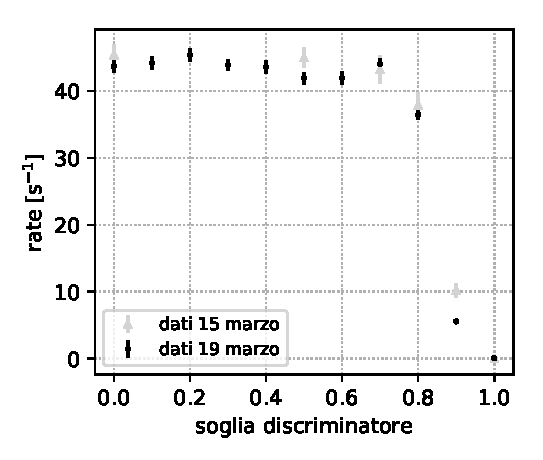
\includegraphics[width=0.6\textwidth]{immagini/soglia}}~
	{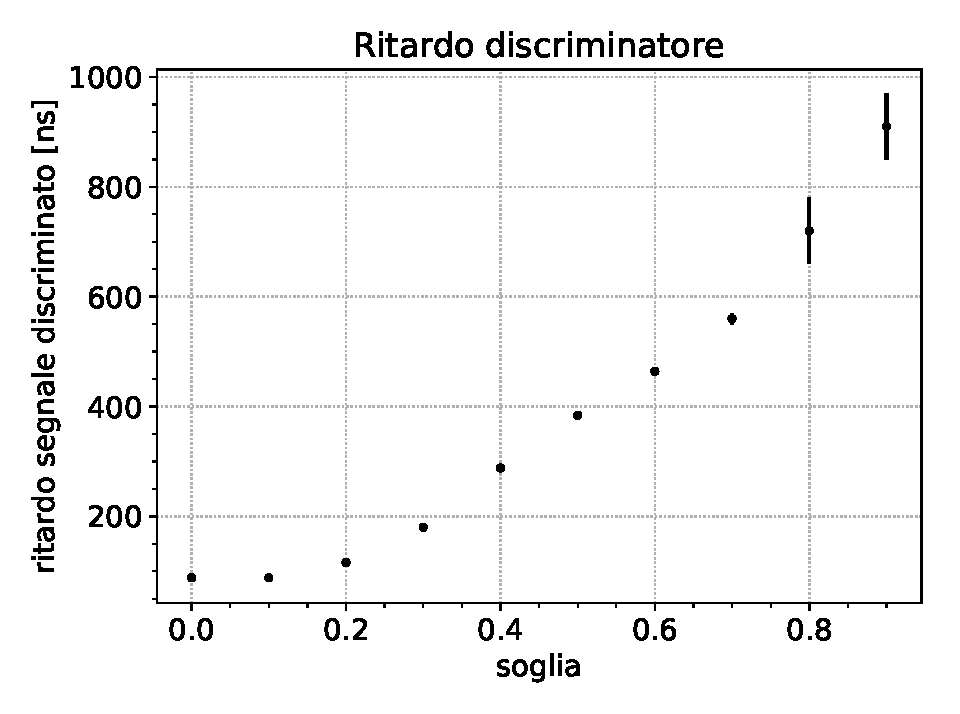
\includegraphics[width=0.6\textwidth]{immagini/ritardo}}
	\caption{\label{fig:sogliaritardo}
	Rate senza bersaglio al variare della soglia del discriminatore (sinistra)
	e ritardo temporale del segnale discriminato rispetto all'ingresso (destra).}
\end{figure}

La manopola di regolazione della soglia del discriminatore non indica l'unità di misura,
però con l'oscilloscopio vediamo che corrisponde circa ai volt quindi supponiamo siano proprio volt.

A \SI0{\degree} senza bersaglio misuriamo il rate al variare della soglia.
Poiché la soglia è in tensione e il segnale del fotodiodo è una curva a campana,
al variare dell'ampiezza del segnale o della soglia
cambia il ritardo del segnale discriminato rispetto a quello in ingresso,
quindi misuriamo anche il ritardo.
Le misure sono riportate in \autoref{fig:sogliaritardo}.
Dal fatto che il ritardo non cambi sulle due soglie più basse
stimiamo che la soglia minima effettiva sia circa \SI{100}{mV}.
Il ritardo introduce un bias verso il basso nelle misure di spettro,
ma non significativo rispetto alla larghezza degli spettri e ad altri problemi esposti di seguito.

% Variamo la soglia del discriminatore collegato al fotodiodo e registriamo il corrispondente rate di eventi a \SI0{\degree} senza collimatori.
% I valori di soglia riportati non hanno unità di misura perché sullo strumento sono solo presenti dei pallini e dei numeri interi.
% Non avendo trovato il manuale dello strumento, ci limitiamo a indicare la posizione del potenziometro.
% Scopriamo (\autoref{fig:soglia}) che il valore della soglia è ininfluente fino a 0.7 e si ha una repentina variazione dopo questo valore.
%
% Per sapere se la soglia ha un effetto minore di quanto misurato dobbiamo aumentare la statistica. I rates misurati hanno (nel migliore dei casi) una precisione del 2\%.
% Siccome il rate diminuisce di molto all'aumentare dell'angolo, le misure ad angoli maggiori avranno un'accuratezza minore. Quindi possiamo affermare che la soglia non avrà alcun effetto sulle misure di rate.
% Pertanto la teniamo a 0 per tutta l'esperienza.
